\chapter{}

\thm{Satz von Arzela-Ascoli}
{
    Sei $\langle X, \mathcal{T}\rangle$ Kompakt und (T2) 
    und $\mathscr{F} \subseteq C(X,\mathbb{R})$
    dann sind folgende Aussagen äquivalent:
    \begin{enumerate}
        \item[(i)] $\mathscr{F}$ ist totalbeschränkt
        \item[(ii)] $\mathscr{F}$ ist punktweise beschränkt 
        (dh.: $\forall x \in X: \underset{f \in \mathscr{F}}{\text{ sup }} |f(x)| < \infty$)
        \item[(iii)] $\mathscr{F}$ ist gleichgradig stetig 
        (dh.: $\forall x \in X \forall \varepsilon > 0 \, \exists U \in \mathcal{U}(x) 
        \forall f \in \mathscr{F}: f(U)\subseteq \mathcal{U}_{\epsilon}(f(x))$)
    \end{enumerate}
}

\begin{myproof}{Satz 9.0.1 ("$(i) \Rightarrow (ii)$")}\\
    Wir betrachten $\mathcal{F}$ Totalbeschränkkt dann erhalten wir die 
        Implikationskette
        \begin{equation*}
            \begin{split}
                &\mathscr{F} \text{ totalbeschränkt }\\
                &\Rightarrow \mathscr{F}\text{ ist beschränkt } \\
                &\Rightarrow sup\{\|f\|_{\infty} : f \in \mathscr{F}\} < \infty \forall x \in X: \mid f(x)\mid \leq \|f\|_{\infty}\\
                &\Rightarrow \mathscr{F} \text{ ist punktweise beschränkt }
            \end{split}
        \end{equation*}
        
        Sei $\varepsilon > 0$ wähle $f_1, \ldots, f_n \in \mathscr{F}$ mit 
        $\mathscr{F} \subseteq \bigcup_{i=1}^{n} \mathcal{U}_{\frac{\varepsilon}{6}}(f_i)$
        Sei $x \in X$. \\
        Wähle für $i = 1, \ldots, n$ ein $U_i \in \mathcal{U}(x)$ so dass
        $\mid f_i(y) - f_i(x) \mid < \frac{\varepsilon}{3}$ für alle $y \in U_i$.\\
        Betrachte $U := \bigcap_{i=1}^{n} U_i $ sei $y \in \mathcal{U} \text{ und } 
        f \in \mathscr{F}$
        weiters wähle $i: f \in \mathcal{U}_{\frac{\varepsilon}{6}}(f_i)$
        $\mid f(y) - f(x) \mid \leq \mid f(y) - f_i(y) \mid + 
        \mid f_i(y) - f_i(x) \mid + \mid f_i(x) - f(x) \mid < \frac{\varepsilon}{6} 
        + \frac{\varepsilon}{3} + \frac{\varepsilon}{6} = \varepsilon$
\end{myproof}

Für die andere Richtung müssen wir ein Lemma einschieben. Also zu dem Zeitpunkt
an dem ich das hier schreibebin ich mir nicht sicher ob wir das Lemma wirklich brauchen. 
Da aber an diese stelle ein Lemma kommt und dannach die andere Richtung bewiesen wird
gehe ich davon aus das es notwendig ist. \\
$\dots$\\
Jetzt habe ich mir das Lemma durchgelesen und es sieht sehr sinnvoll aus.

\mlenma{}
{
    Sei $\langle\Omega, d\rangle$ ein metrischer Raum und es gelte:
    \begin{equation*}
    \begin{split}
        \forall \epsilon > 0 \exists \langle \Omega', d' \rangle \text{ metrischer Raum },
        &\Phi : \Omega \to \Omega',
        \delta>0: \Phi(\Omega) \text{ ist Totalbeschränkkt }\\
        \forall x,y \in \Omega: &d'(\Phi(x),\Phi(y)) < \delta 
        \Rightarrow d(x,y)< \epsilon
    \end{split}
    \end{equation*}
    Dann folgt $\rangle \Omega, d \langle$ ist totalbeschränkt
}
     
\begin{proof}{Lemma 9.0.2}\\
    Sei $\epsilon > 0$ wähle $\langle \Omega', d' \rangle, \Phi, \delta$ so dass
    die Voraussetzungen des Lemmas erfüllt sind.
    Wähle $x_1', \ldots, x_n' \in \Omega'$ mit
    $\Phi(\Omega) \subseteq \bigcup_{i=1}^{n} 
    \underbrace{\Phi^{-1} (\mathcal{U}_{\delta}(x_i))}_{\subseteq \mathcal{U}_{\epsilon}(x-i)}$
    Sei $y \in \Phi^{-1}(\mathcal{U}_{\delta}(x_i))$
    dann gilt $d'(\Phi(y), \Phi(x_i)) < \delta$ und somit $d(y,x_i) < \epsilon$
    
\end{proof}
Nachdem wir das Lemma bewiesen haben können wir die Rückrichtnung antreten.

\begin{proof}{Satz 9.0.1 ("$(ii) \Rightarrow (i)$")}\\
    Sei $\varepsilon > 0$. Für $x \in X$ wähle $ U_x \in \mathcal{U}(x)$ so dass
    $\forall y \in U_x \forall f \in \mathscr{F}: |f(y) - f(x)| < \varepsilon$
    ohne Beschränkung der Allgemeinheit sei $U_x$ offen.
    Da $X$ kompakt ist gibt es $x_1, \ldots, x_n \in X$ so dass
    $X = \bigcup_{i=1}^{n} U_{x_i}$
    Definiere die Abbildung
    $$ 
    \Phi:\begin{cases}
         \mathscr{F} \to \mathbb{R}^n\\
        f \mapsto (f(x_1), \ldots, f(x_n))
    \end{cases}
    $$
    \begin{itemize}
        \item $\Phi(\mathscr{F}):= \{(f(x_1), \ldots, f(x_n)) : f \in \mathscr{F}\}$
        ist beschränkt in $\mathbb{R}^n$ da $\mathscr{F}$ punktweise beschränkt ist.
        Somit ist $\Phi(\mathscr{F})$ totalbeschränkt in $\mathbb{R}^n$.
        \item Setze $\delta := \frac{\epsilon}{3}$
        Sei $f,g \in \mathscr{F}$ mit $\|\Phi(f)-\Phi\|\leq \delta$
        $\Rightarrow |f(x_i) - g(x_i)| < \delta$ für $i \in \{1, \ldots, n\}$
        Wähle $x \in X$ und $i$ so dass für $x \in U_{x_i}$ gilt 
        $\mid f(x) - g(x) \mid \leq 
        \underbrace{\mid f(x)-f(x_i)\mid}_{< \epsilon} 
        + \underbrace{\mid f(x_i)-g(x_i)}_{\delta = \frac{\epsilon}{2}}
        +\underbrace{\mid g(x)-g(x_i)\mid}_{< \epsilon}$
        $< \epsilon + \frac{\epsilon}{3} + \epsilon = \frac{7\epsilon}{3}$
        Also gilt $\|f-g\|_{\infty} < \frac{7\epsilon}{3}$ 
        $\overset{\text{Lemma 9.0.2}}{\Rightarrow}$ $\mathscr{F}$ ist totalbeschränkt
    \end{itemize}
\end{proof}

\ex{}
{
    Sei $\alpha \in (0,1], L>0, C>=$
    $$
    \mathcal{F}_{\alpha,L,C}:= \{ f : [0,1] \to \mathbb{R}
    \mid f \text{ ist Lipschitz-stetig mit Exponent } \alpha 
    \text{ und Lipschitzkonstante L}\}.
    $$
    Dann ist $\mathcal{F}_{\alpha,L,C}$ total beschränkt.
    \begin{itemize}
        \item $|f(x)| \leq |f(x)-f(0)| + |f(0)| \leq L|x-0|^\alpha + C \leq L+C \leq \epsilon$
        \item $|f(x)-f(y)| \leq L|x-y|^{\alpha}$ Sei $\varepsilon > 0$. 
        $|x-y| < \left(\frac{\varepsilon}{L}\right)^{1/\alpha}: |f(y)-f(x)| < \varepsilon$
    \end{itemize}
    $f:[0,1] \to \mathbb{R}$ stetig.\\
    Gewisse Funktionen lassen sich als Potenzen darstellen.
    $$
    f(x) = \sum_{n=0}^{\infty} a_n x^n = \lim_{N \to \infty} 
    \underbrace{\sum_{n=0}^{N} a_n x^n}_{\text{Polynom }\mathbb{P}_N}
    $$
}

\thm{Weierstraßesscher Approximationssatz}
{
    Sei $f:[a,b] \to \mathbb{R}$ stetig. Dann gibt es eine Folge von Polynomen
    $(P_n)_{n \in \mathbb{N}}$ so dass 
    $$
    \lim_{n \to \infty} \|f - P_n\|_{\infty} = 0
    $$
    $\langle C(X,\mathbb{R}), \|\cdot\|_{\infty}\rangle$ wobei 
    $\langle X, \mathcal{T} \rangle$ kompakter Topologischer-Raum. \\
    $\mathcal{A}\subseteq C(X,\mathbb{R})$
}

\thm{Stone-Weierstraß}
{
    Sei $\langle X, \mathcal{T} \rangle$ kompakter Topologischer-Raum und 
    $\mathcal{A} \subseteq C(X,\mathbb{R})$ eine Unteralgebra die
    \begin{enumerate}
        \item die Niergends verschwindend ist, dh.: $\forall x \in X \, \exists f \in \mathcal{A}: f(x) \neq 0$
        \item Punkte trennend 
        dh.:$ \forall x,y \in X, x \neq y \, \exists f \in \mathcal{A}: f(x) \neq f(y)$
    \end{enumerate}
    Dann ist $\mathcal{A}$ dicht in $C(X,\mathbb{R})$ 
    (dh.: $\overline{\mathcal{A}} = C(X,\mathbb{R})$).
}

\mlenma{}
{
    Sei $X$ ein kompakter topologischer Raum und 
    $\mathcal{A} \subseteq C(X,\mathbb{R})$ eine Unteralgebra die 
    \begin{enumerate}
        \item die Niergends verschwindend ist, dh.: $\forall x \in X \, \exists f \in \mathcal{A}: f(x) \neq 0$
        \item Punkte trennend 
        dh.:$ \forall x,y \in X, x \neq y \, \exists f \in \mathcal{A}: f(x) \neq f(y)$
    \end{enumerate}
    Dann gilt: $1 \in \overline{\mathcal{A}}^{\|\cdot\|_{\infty}}$
}

\begin{proof}{Lemma 9.0.3}\\
    \begin{itemize}
        \item[(1.)] Wir zeigen:$\exists f \in \mathcal{A} \forall x \in X; f(x)>0$
        Sei $ x \in X \,$ 
        wähle $f_x \in \mathcal{A}$ mit $f_x(x) \neq 0$.
        Wähle $\mathcal{O}_x \in \mathscr{U}(x)$ oofen.
        so dass $f_x(y) \neq 0$ für alle $y \in \mathcal{O}_x$.
        Da $X$ kompakt gibt es $x_1, \ldots, x_n \in X$ so dass
        $X = \bigcup_{i=1}^{n} \mathcal{O}_{x_i}$
        Definiere $f := \sum_{i=1}^{n} f_{x_i}^2 \Rightarrow f \in \mathcal{A}$
        Sei $x \in X$ dann gibt es $i \in \{1, \ldots, n\}$ so dass
        $x \in \mathcal{O}_{x_i} \Rightarrow f_{x_i}(x) \neq 0 
        \Rightarrow f(x) =\sum_{i=1}^{n} f_{x_i}(x) \geq  f_{x_i}^2(x) > 0$
        \item[(2.)] Wir zeigen: $1 = (1-t)\sum_{n=0}^{N}t^n + t^{N+1}$ d.h.: 
        $1 = s\sum_{n=0}^{N}(1-s)^n + (1-s)^{N+1} \forall s \in \mathbb{R}$
        Wähle $f \in \mathcal{A}$ mit $\delta > 0 \forall x \in X: \delta \geq f(x)\leq 1$. 
        \nt{
             Wir können das das f so wegen (1-) wählen
             Seit $f(x)$ wie in (1.) Setze $\tilde{f} := \frac{f}{\|f\|_{\infty}}\underbrace{min_{x \in X}\{f(x)\}}_{>0}$
             Weil X kompakt ist existiert das Minimum und ist überall größer als 0.
        }
             $\Rightarrow 1 = \underbrace{f(x)\sum_{n=0}^{N}(1-f(x))^n}_{\in \mathcal{A}}+
            \underbrace{(1-f(x))^{N+1}}_{0\leq -1-\delta < 1}$ also 
            $|(1-f(x))^{N+1}| < (1-\delta)^{N+1}\to 0 \Rightarrow
             \underset{n\to \infty}{lim}$ Gelcihmäßig
    \end{itemize}
\end{proof}

\nt{
    Für den Beweis von Satz von Stone-Weierstraß kann man ohne Beschränkung der Allgemeinheit
    annehmen dass $1 \in \mathcal{A}$ (wegen Lemma 9.0.6).
}

\begin{proof}
    Sei $\mathcal{A}$ Wie in Satz von Stone-Weierstraß. Betrachte $\mathcal{B}:=span(\mathcal{A}\cup \{1\})$
    Dann ist $\mathcal{B}$ eine Unteralgebra das bedeutet ($(\sum_{endl.}\alpha_i f_i + \alpha 1)(\sum_{endl.}\beta_i g_i + \beta 1) = [\cdots] \in \mathcal{A}$) für die gilt:
    \begin{enumerate}
        \item $\mathcal{B}$ ist Punkte trennend.
        \item $1 \in \mathcal{B}$

        \item $\mathcal{B}$ ist nirgends verschwindend.
    \end{enumerate}
    $\underset{\text{Spezialf. v. Satz}}{\Longrightarrow} \overline{\mathcal{B}}= C(X,\mathbb{R})$
    $1 \in \overline{\mathcal{A}}$ Wegen Lemma 9.0.3.gilt: damit auch 
    $\overline{\mathcal{A}} = C(X,\mathbb{R})$ 
\end{proof}

\mlenma{}
{
    Sei $\mathcal{A}\subseteq C(X,\mathbb{R})$ eine Punktetrennende Unteralgebra mit 
    $1 \in \mathcal{A} z\in X, A \subseteq X$ Abgeschlossen mi $z \notin A$
    $$
    \Rightarrow \exists V \in \mathcal{U}(z)\text{ offen } : V \cap A \neq \emptyset
    $$
    und $\forall \epsilon > 0 \, \exists f \in \mathcal{A}$ so dass
   \begin{equation*}
    \begin{split}
        \forall x \in X: &|f(x)| \leq 1\\
        \forall x \in V: &|f(x)| \leq \epsilon\\
        \forall x \in A: &|f(x) |\geq 1 - \epsilon
    \end{split}
\end{equation*}
}
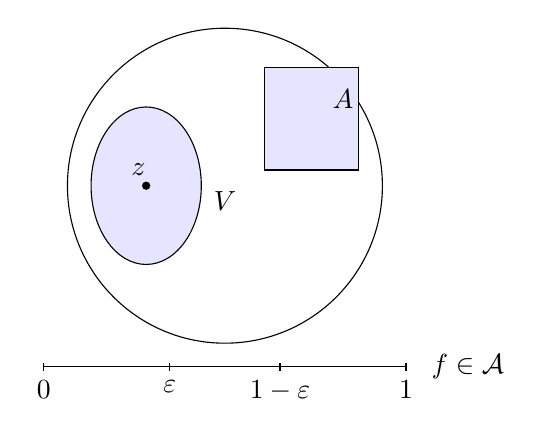
\begin{tikzpicture}[scale=1]

  % großer Kreis
  \draw (0,0) circle (2cm);

  % Ellipse um z
  \draw[fill=blue!10] (-1,0) ellipse (0.7cm and 1cm);
  \fill (-1,0) circle (1.5pt);
  \node at (-1.1,0.2) {$z$};

  % Rechteck A
  \draw[fill=blue!10] (0.5,0.2) rectangle (1.7,1.5);
  \node at (1.5,1.1) {$A$};

  % V im Inneren
  \node at (0,-0.2) {$V$};

  % Achse unten: 0, epsilon, 1-epsilon, 1
  \draw (-2.3,-2.3) -- (2.3,-2.3);

  % Ticks
  \draw (-2.3,-2.25) -- (-2.3,-2.35);   % 0
  \draw (-0.7,-2.25) -- (-0.7,-2.35);   % eps
  \draw (0.7,-2.25) -- (0.7,-2.35);     % 1-eps
  \draw (2.3,-2.25) -- (2.3,-2.35);     % 1

  % Beschriftungen
  \node[below] at (-2.3,-2.35) {$0$};
  \node[below] at (-0.7,-2.35) {$\varepsilon$};
  \node[below] at (0.7,-2.35) {$1-\varepsilon$};
  \node[below] at (2.3,-2.35) {$1$};

  % f \in A
  \node[right] at (2.5,-2.3) {$f \in \mathcal{A}$};

\end{tikzpicture}

\begin{proof}{Lemma 9.0.7}\\
   \begin{itemize}
    \item[(1.)] Wir zeigen: $\exists h \in \mathcal{A}$ so dass
    $\forall x \in X: h(x) \geq 0, h(z) = 0, \forall x \in A: h(x) > 0$\\
    Konstruiere $h \in \mathcal{A}$, $\varepsilon \in (0,1)$, $V \in U(x)$ offen. 
    $\forall x \in V: h(x) < \frac{\varepsilon}{3}$ und 
    $\forall x \in A: h(x) > \delta$ 
    und $\forall x \in X: 0 \le h(x) \le 1$.

    Für $y \in A$ wähle $g_y \in \mathcal{A}$ : 
    $g_y(y) \neq 0$ und $g_y(z) = 0$.

    Setze 
    $$
        h_y = \frac{1}{\|g_y\|_\infty^2}\, g_y^2 \in \mathcal{A}.
    $$
    Dann gilt 
    $$
        h_y \in \mathcal{A},\quad h_y(y) > 0,\quad 
        h_y(z) = 0,\quad 
        \forall x \in X: 0 \le h_y(x) \le 1.
    $$

    Setze $O_y := \{x \in X \mid h_y(x) > 0\}$
    offen, und $y \in O_y$.

    $A \subseteq \bigcup_{y \in A} O_y 
    \Rightarrow$ Wähle $y_1,\dots, y_n \in A$:
    $$
        A \subseteq \bigcup_{i=1}^n O_{y_i}.
    $$

    Setze 
    $h := \frac{1}{n}\sum_{i=1}^n h_{y_i}.$

    $$ \Rightarrow
        h \in \mathcal{A},\quad 
        \forall x \in X: 0 \le h(x) \le 1,\quad 
        h(z) = 0.
    $$

    Sei $x \in A$. Wähle $j$ mit $x \in O_{y_j}$. Dann
    $$
        h(x) 
        = \frac{1}{n}\sum_{i=1}^n h_{y_i}(x)
        \ge \frac{1}{n} h_{y_j}(x)
        > 0.
    $$

    $$ \Rightarrow
        \delta := \min_{x \in A} h(x) > 0,
        \qquad 
        V := \{x \in X \mid h(x) < \tfrac{\varepsilon}{3}\}.
    $$
    \item[(2.)] Wir zeigen:$\dots$
    \end{itemize}
\end{proof} 